\documentclass[a4paper]{article}

\usepackage[english]{babel}
\usepackage[utf8]{inputenc}
\usepackage{amsmath}
\usepackage{graphicx}
\usepackage[colorinlistoftodos]{todonotes}
\usepackage[useregional]{datetime2}
\usepackage{fancyhdr}
\usepackage{titlesec}
\usepackage{listings} 
\usepackage{hyperref}
\hypersetup{
    colorlinks=true,
    linkcolor=blue,
    filecolor=magenta,      
    urlcolor=blue,
}
\usepackage{caption}
\usepackage{titling}

\usepackage{color}

 \usepackage{wrapfig}

\setcounter{secnumdepth}{4}

\setlength{\droptitle}{-4em}

\setlength{\intextsep}{6pt plus 2pt minus 2pt}


%Project Title
\newcommand{\projectTitle}{Tic-Tac-Toe}
%Homework Number
\newcommand{\assignmentNumber}{1}

%Submission date goes here.
%Format: #Day of Month #Hour:#Minute AM/PM
\newcommand{\projectDate}{3rd of March 11:59 PM}

%Contact to reach.
\newcommand{\contactName}{Hasan Can Aslan}
\newcommand{\contactMail}{haslan16@ku.edu.tr}

%Define colors as shown below to use in text.
\definecolor{Red}{RGB}{255, 0, 0}
\definecolor{Green}{RGB}{0, 255, 0}
\definecolor{Blue}{RGB}{0, 0, 255}

\author{Hasan Can Aslan}

\title{\projectTitle}

\date{Submission Date: \projectDate}

\begin{document}

\maketitle

\lstset{language=Python}
\pagestyle{fancy}
\fancyhf{}
\chead{\projectTitle}
\rhead{Assignment \#\assignmentNumber}
\lhead{KOLT Python}
\lfoot{\nouppercase{\leftmark}}
\rfoot{Page \thepage}
\thispagestyle{fancy}
\renewcommand{\headrulewidth}{0.4pt}
\renewcommand{\footrulewidth}{0.4pt}


\section{Introduction}

On this project, your challenge in this exercise is to implement the classical Tic-Tac-Toe game logic using Python, and a graphical visualization using the \texttt{turtle} module to make a two-player game that you can play with a friend.

%Do not change this section.
\subsection{Submission}
We will use \emph{\href{https://okpy.org}{OK}}

%Do not change this section.
\subsection{Academic Honesty}
Koç University's \emph{\href{https://vpaa.ku.edu.tr/sites/vpaa.ku.edu.tr/files/Misc_Documents/Statement_on_Academic_Honesty.pdf}{Statement on Academic Honesty}} holds for all the homework given in this course. Failing to comply with the statement will be penalized accordingly. If you are unsure whether your action violates the code of conduct, please consult with your instructor.

%TODO: Write aim of the project
\subsection{Aim of the Project}
In your homework assignments, the \textbf{functionality} and \textbf{style} of your programs are \textbf{both important.}  A program that “works” is not necessarily a good program. A good program is \textbf{comprehensible, readable and well structured.} Therefore you’re expected to decompose the main problem into simpler subtasks and \underline{\textbf{implement helper functions}} for these subtasks. You’re also expected to write comments if needed, be careful about indentation and use descriptive names for helper functions. Even if your program functions well according to the project requirements, you can still improve your code style and how you decompose the task.

%Do not change this section.
\subsection{Given Code}
This part is \textbf{optional} but advised as it will allow you to understand the given partitions of the code better. The code given to you has commented above all the functions. Below are the functions are given to you in the code with their explanation.

\newpage
%Explain the functions you have given in this section.
%Examples are given below.
\subsubsection{Given Functions}
\label{themeMethod}
%This is a list. Lists always begin with this tag. "itemize" describes the list, not begin.
\begin{itemize}

%This is a list item. There is no need to indicate the end for an item as it ends at the next item tag.

\item
\begin{lstlisting}
def draw_empty_board():
\end{lstlisting}
This function should draw the \textbf{empty Tic-Tac-Toe board} using turtle module.

\item
\begin{lstlisting}
def draw_x_in_square(row, column):
\end{lstlisting}
This function should draw a \textbf{X symbol} on the given square of tic-tac-toe board.

\item
\begin{lstlisting}
def draw_o_in_square(row, column):
\end{lstlisting}
This function should draw an \textbf{O symbol} on the given square of tic-tac-toe board.

\item
\begin{lstlisting}
def display_setup():
\end{lstlisting}
Sets the \textbf{display} i.e. screen size, animation speed.

\item
\begin{lstlisting}
if __name__ == '__main__':
\end{lstlisting}
'\_main' is the name of the scope in which top-level code executes. You do not have to fully understand the benefits of writing your code under if \_\_name\_\_ == '\_\_main\_\_' block for now. We will discuss its meaning when we are talking about Python packages and modules. For now, just think of this as the main entry to your program.


\end{itemize}

%Do not change this section.
\subsubsection{Given Constants}
Five constants: SCREEN\_WIDTH, SCREEN\_HEIGHT, PEN\_SIZE, SQUARE\_SIZE and ANIMATION\_SPEED are given at the top of the project. You will use these constants as \textbf{arguments} for configuring the screen and turtle. Since you did not learn functions in detail yet, \textbf{we will provide necessary code in corresponding sections of the project.}

%Do not change this section.
\subsection{Further Questions}
For further questions \textbf{about the project} you may contact \textbf{\contactName} at \href{mailto:\contactMail}{\mbox{[\contactMail]}}. Note that it may take up to 24 hours before you receive a response so please ask your questions \textbf{before} it is too late. No questions will be answered when there is \textbf{less than two days} left for the submission.

%This allows you to start a new page regardless of where the previous page ends. Please try to separate sections properly. However, refrain from leaving extensive amounts of blank space as this may cause the students to think that the project file ends there.
\newpage

\section{Project Steps}
\label{worlds}

%This is a figure. image.png is the path of the image file that will be used.
% \begin{figure}[!htb]
% \centering
% \includegraphics[width=1\textwidth]{worlds.png}
% \caption{Worlds given at project.}\label{fig:worlds}
% \end{figure}

%Number of task groups and tasks are dependent on the project. Feel free to change accordingly.
\subsection{Displaying Empty Board}
Let's start to draw! Our first step is drawing an empty Tic-Tac-Toe board using the turtle module. To do that you should fill the given function:
\begin{lstlisting} 
def draw_empty_board():
\end{lstlisting}

\begin{figure}[!htb]
\centering
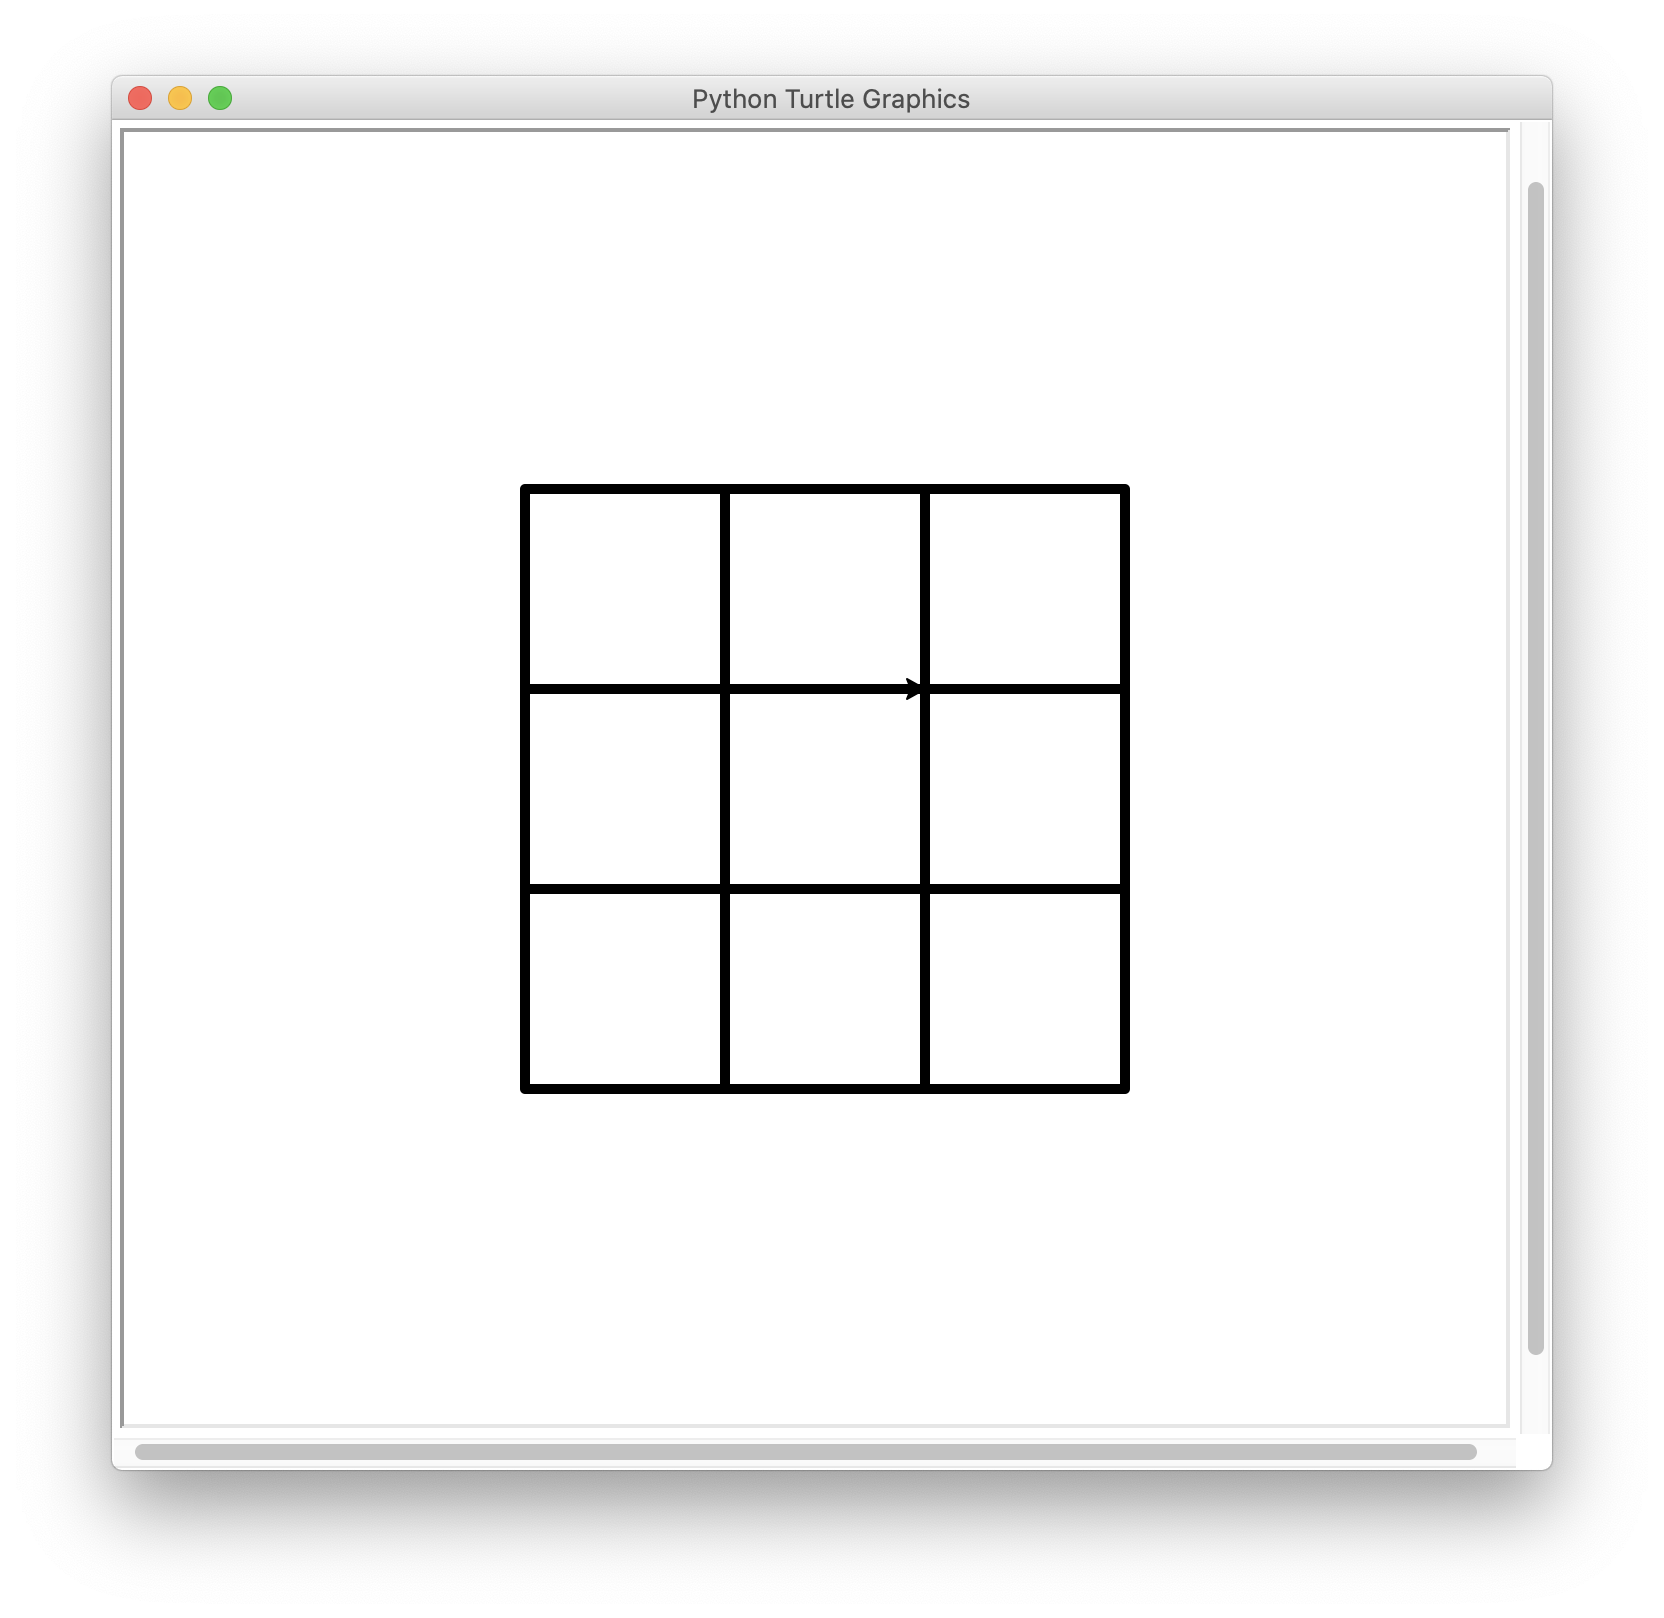
\includegraphics[width=1\textwidth]{empty_board.png}
\caption{Empty board.}\label{fig:outputs}
\end{figure}

\textbf{Hints:}
\begin{enumerate}
\item You might want to implement a helper function for drawing only one square.
\item You can create a "nested" for loop to draw a 3x3 board using the helper function you created.
\end{enumerate}

\newpage
\subsection{Drawing X}
Now you are warmed up. Drawing two more lines should be a piece of cake for you. This function should draw an X symbol, here is the trickier part, you should draw X on the given square of the Tic-Tac-Toe board. Takes two arguments, row and column numbers for X to be drawn. You need to fill the given function:

\begin{lstlisting} 
def draw_x_in_square(row, column):
\end{lstlisting}

\begin{figure}[!htb]
\centering
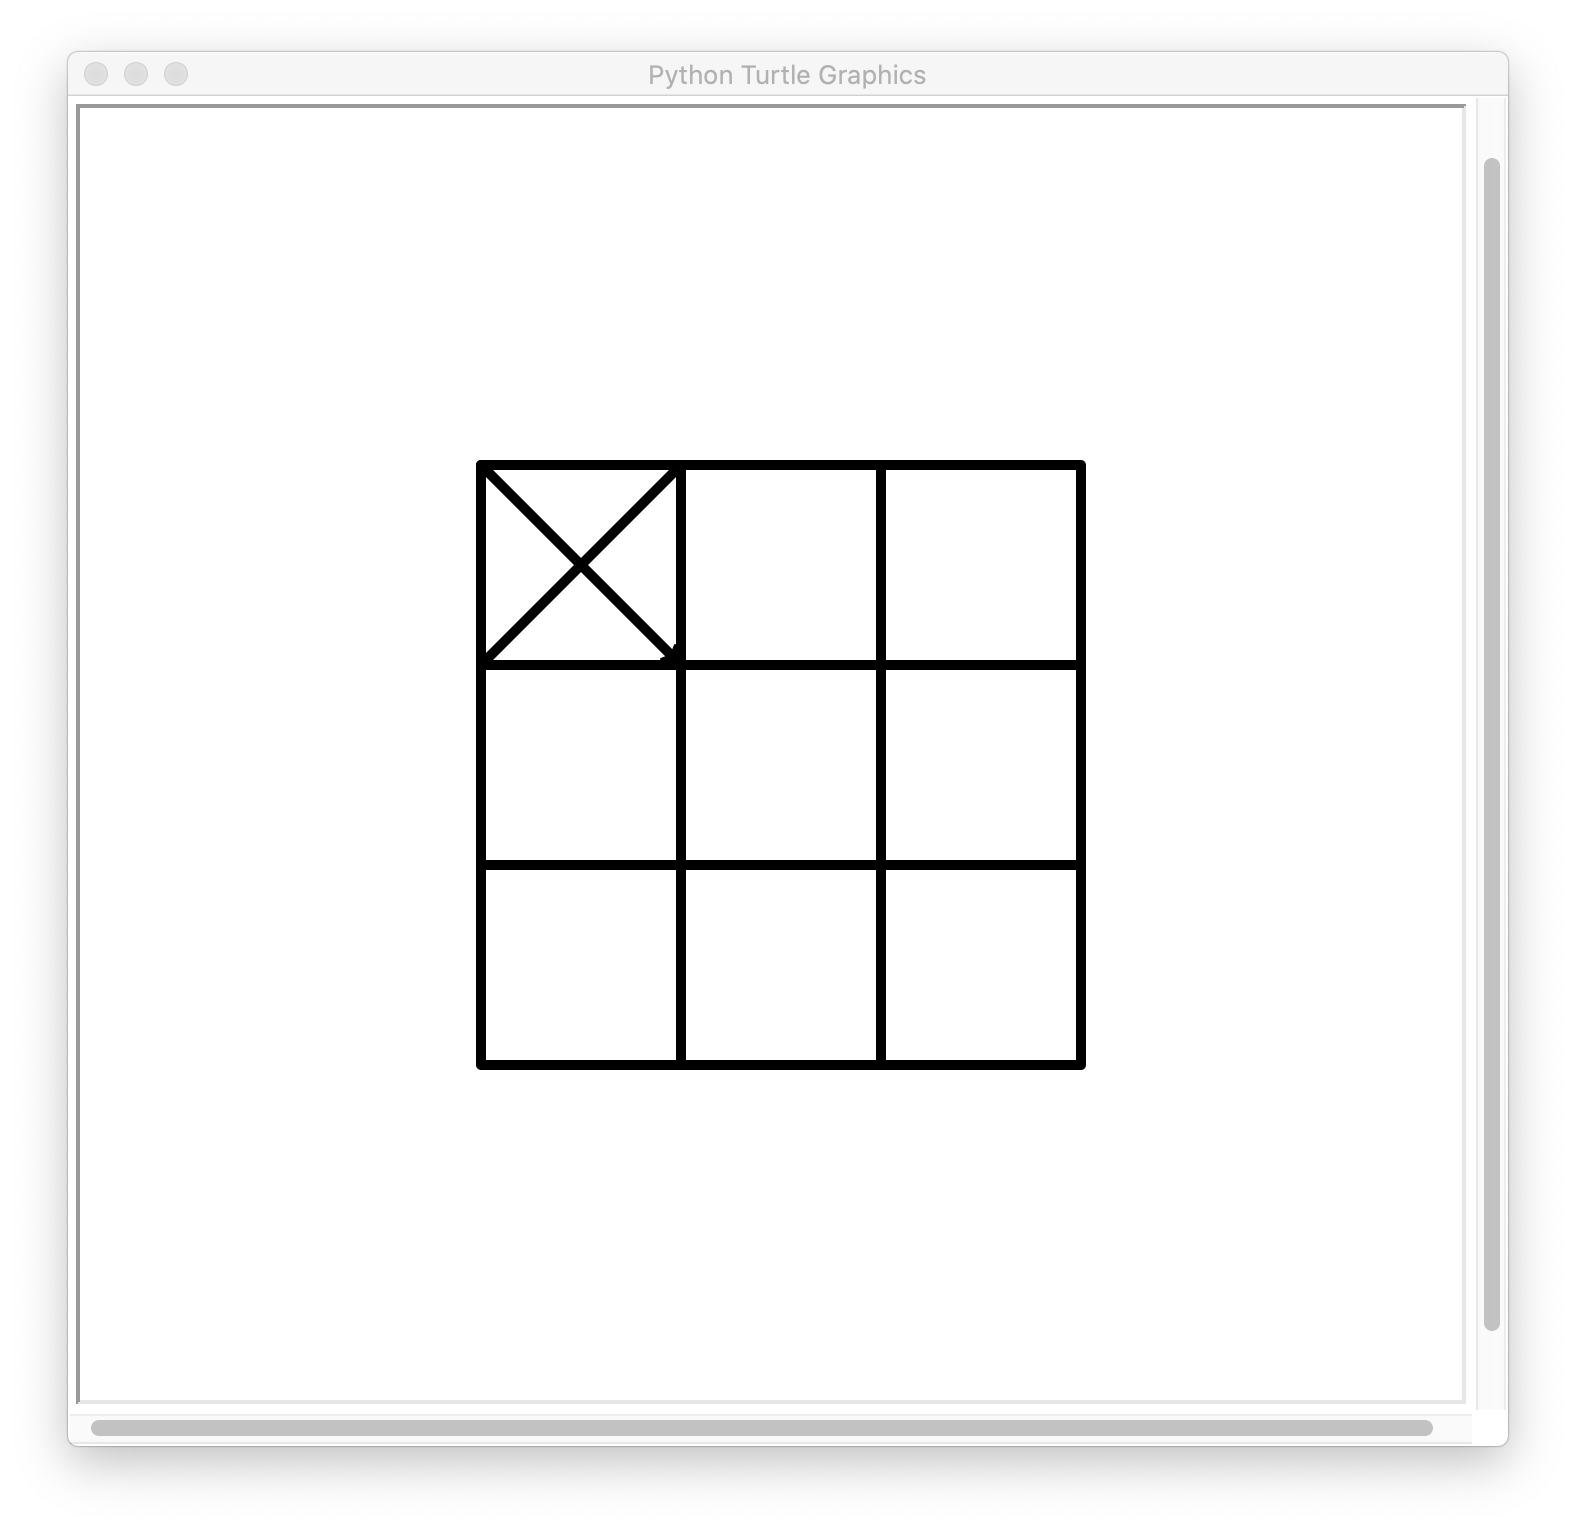
\includegraphics[width=1\textwidth]{x_drawing.png}
\caption{X drawing on board.}\label{fig:outputs}
\end{figure}

\textbf{Hints:}
\begin{enumerate}
\item You might want to use penup, pendown, setpos, setheading, forward functions from the turtle module.
\item We recommend you to spend some time with turtle module in the interactive shell to understand how it uses coordinates (which directions are positive, which angles correspond to which directions, etc.)
\end{enumerate}

\newpage
\subsection{Drawing O}
Very well, Let's bend these lines! This function is very alike to the previous one only difference is its shape. You should draw an O symbol on the given square of the Tic-Tac-Toe board. Takes two arguments, row and column numbers for O to be drawn. You need to fill the given function:

\begin{lstlisting} 
def draw_o_in_square(row, column):
\end{lstlisting}

\begin{figure}[!htb]
\centering
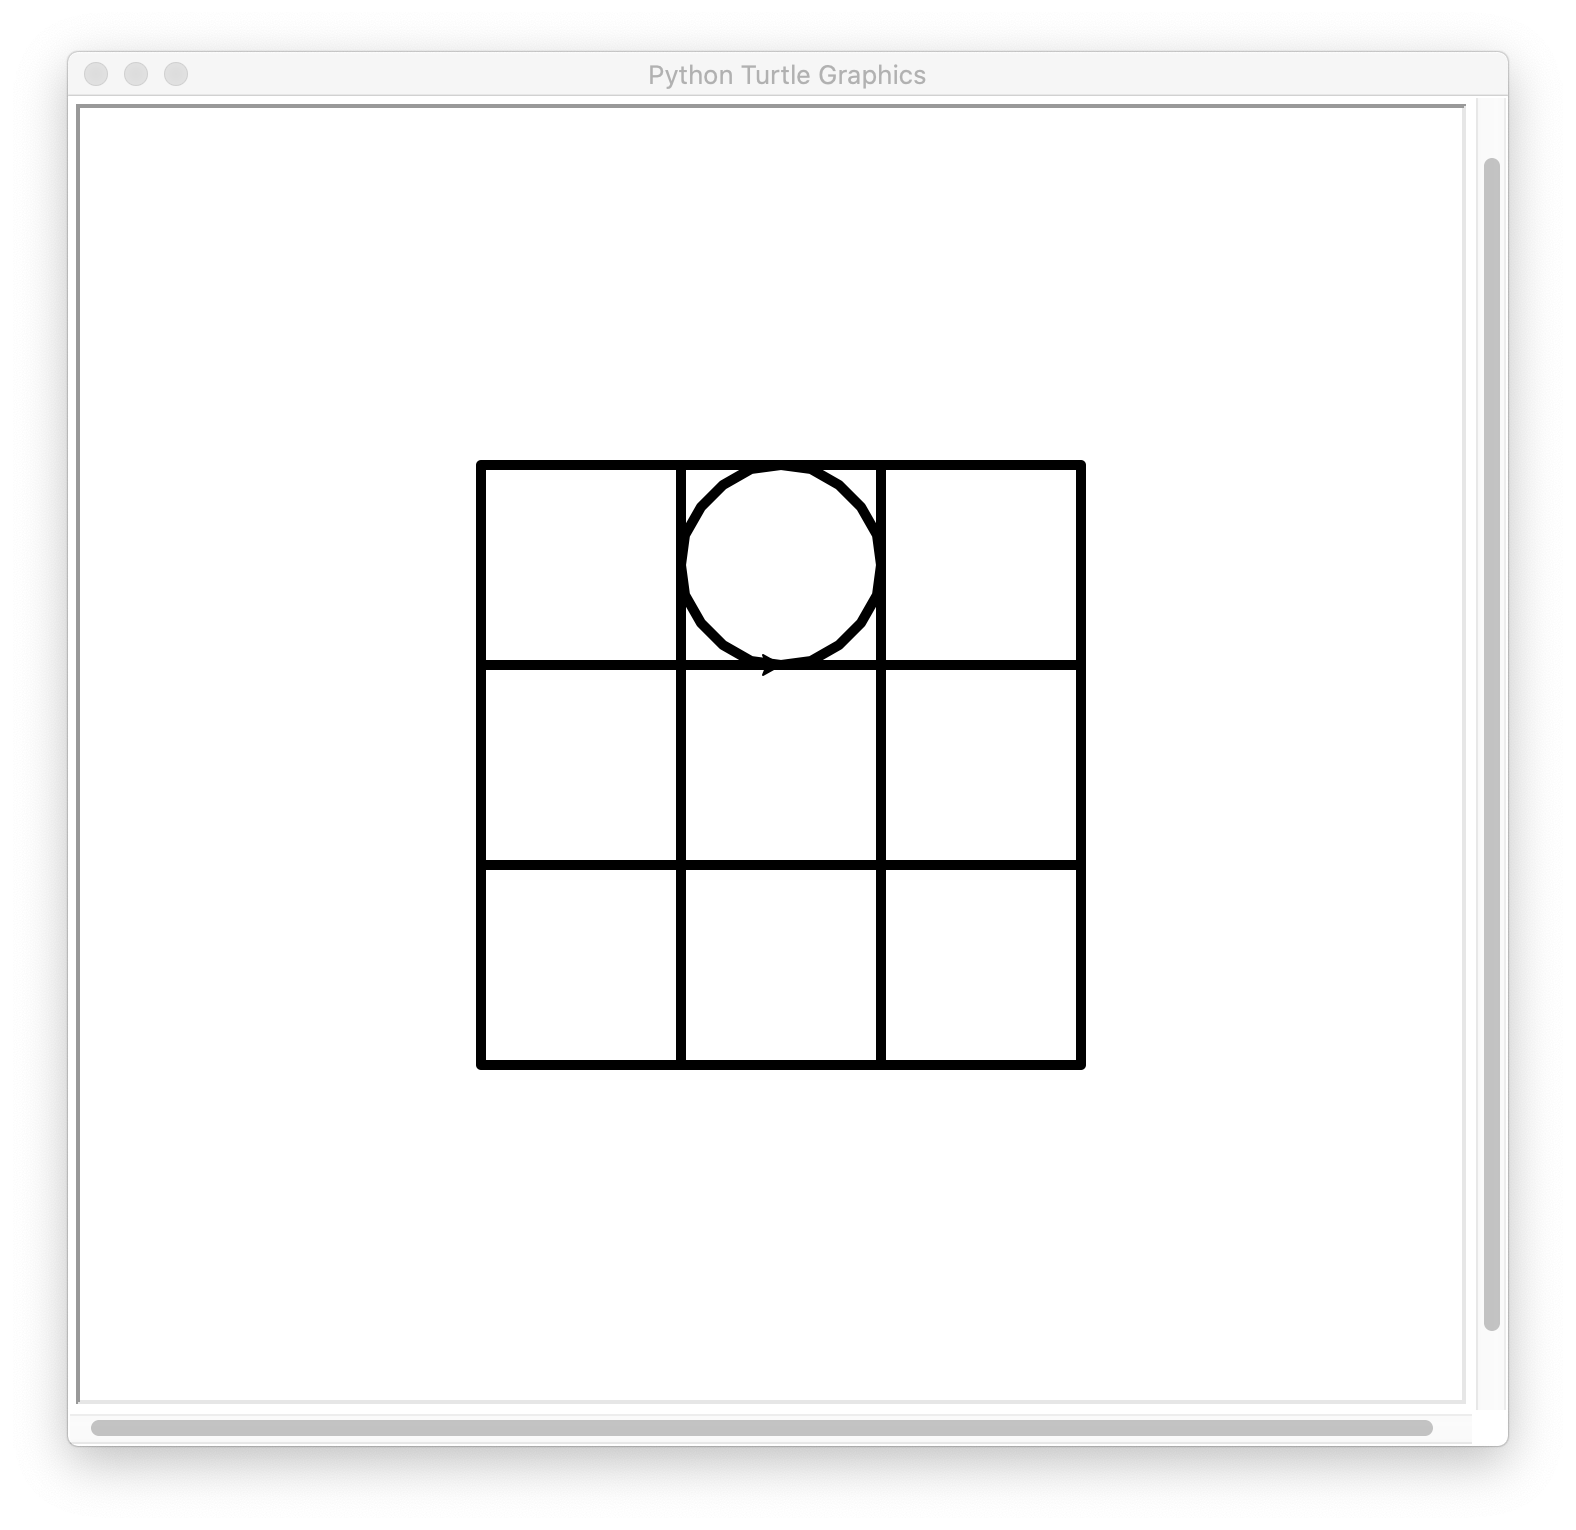
\includegraphics[width=1\textwidth]{o_drawing.png}
\caption{O drawing on board.}\label{fig:outputs}
\end{figure}


\textbf{Hints:}
\begin{enumerate}
\item You might want to use penup, pendown, setpos, setheading, circle functions from the turtle module.
\item We recommend you to spend some time with turtle module in the interactive shell to understand how it uses coordinates (which directions are positive, which angles correspond to which directions, etc.)
\end{enumerate}

\newpage
\subsection{Taking Player's Names}
You've done great so far! Now, you should take players' names, assign them to \textit{player\_names} list. Any string other than an empty string is considered a valid name.

\begin{lstlisting} 
player_names = []
\end{lstlisting}

\begin{figure}[!htb]
\centering
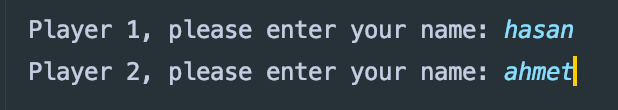
\includegraphics[width=1\textwidth]{enter_name.png}
\caption{Enter name prompt.}\label{fig:outputs}
\end{figure}

\subsection{Getting Current Player}
You should get current player's name to play, assign it to \textit{current\_player\_name} variable.

\begin{lstlisting} 
current_player_name = ''
\end{lstlisting}


\subsection{Taking Player's Move}
Let's begin to play! The next step is to deal with handling user input. When a player (say player 1, who is X) wants to place an X on the screen, they can’t just click on a screen. So we are going to approximate this clicking simply by asking the user for a coordinate of where they want to place their piece. Get where the user wants to place X or O. Feel free to choose which user to put which sign. Assign it to \textit{move} variable for checking.

\begin{lstlisting} 
move = ''
\end{lstlisting}

\begin{figure}[!htb]
\centering

\includegraphics[width=1\textwidth]{user_move.png}
\caption{Taking player's move.}\label{fig:outputs}
\end{figure}

\newpage
\subsection{Validating the Move}
You must validate the user's move. Don’t worry about checking whether someone won the game at this part, but if a player tries to put a piece in a game position where there already is another piece, do not allow the piece to go there. If the move is invalid, you need to ask again until the user enters a valid move.
\\
\begin{figure}[!htb]
\centering
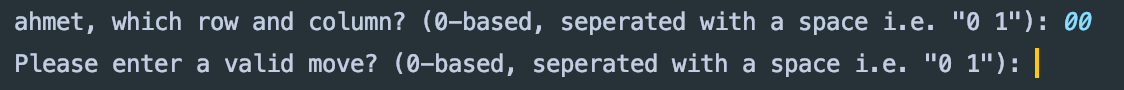
\includegraphics[width=1\textwidth]{invalid_input.png}
\caption{Invalid input.}\label{fig:outputs}
\end{figure}

\textbf{Hints:}
\begin{enumerate}
\item It should be a string consisting of two parts (Hint: use "string".split(' ') function)
\item Both its parts should be integers (Hint: "string".isnumeric() function)
\item Integers should be in range [0, 2] inclusive.
\item Selected square should be empty.
\end{enumerate}


\subsection{Playing the Move}
It's time to play the move! There are two things to do: modifying the \textit{game} list and display the move using the turtle. You should use the functions for drawing X and O that you created earlier in this project. \newline

\textbf{Hint:}
\begin{itemize}
\item
Game of Tic-Tac-Toe is represented as a list of lists, like so: \newline
game = [[X, O, X], [O, X, O], [O, X, X]]
\end{itemize}

\subsection{Checking Win Conditions}
Now, after the user plays his/her move you need to check there is a win condition holds. Your challenge in this part is checking conditions and assign result (True or False) to \textit{there\_is\_winner} variable. If the user wins, terminate the loop and if there is a winner, and show a congratulatory message on the console. If there is no winner at the end of the game (\textit{there\_is\_winner} variable is still False), given code prints \text ''Tie''.

\begin{lstlisting} 
there_is_winner = False
\end{lstlisting}

\begin{figure}[!htb]
\centering
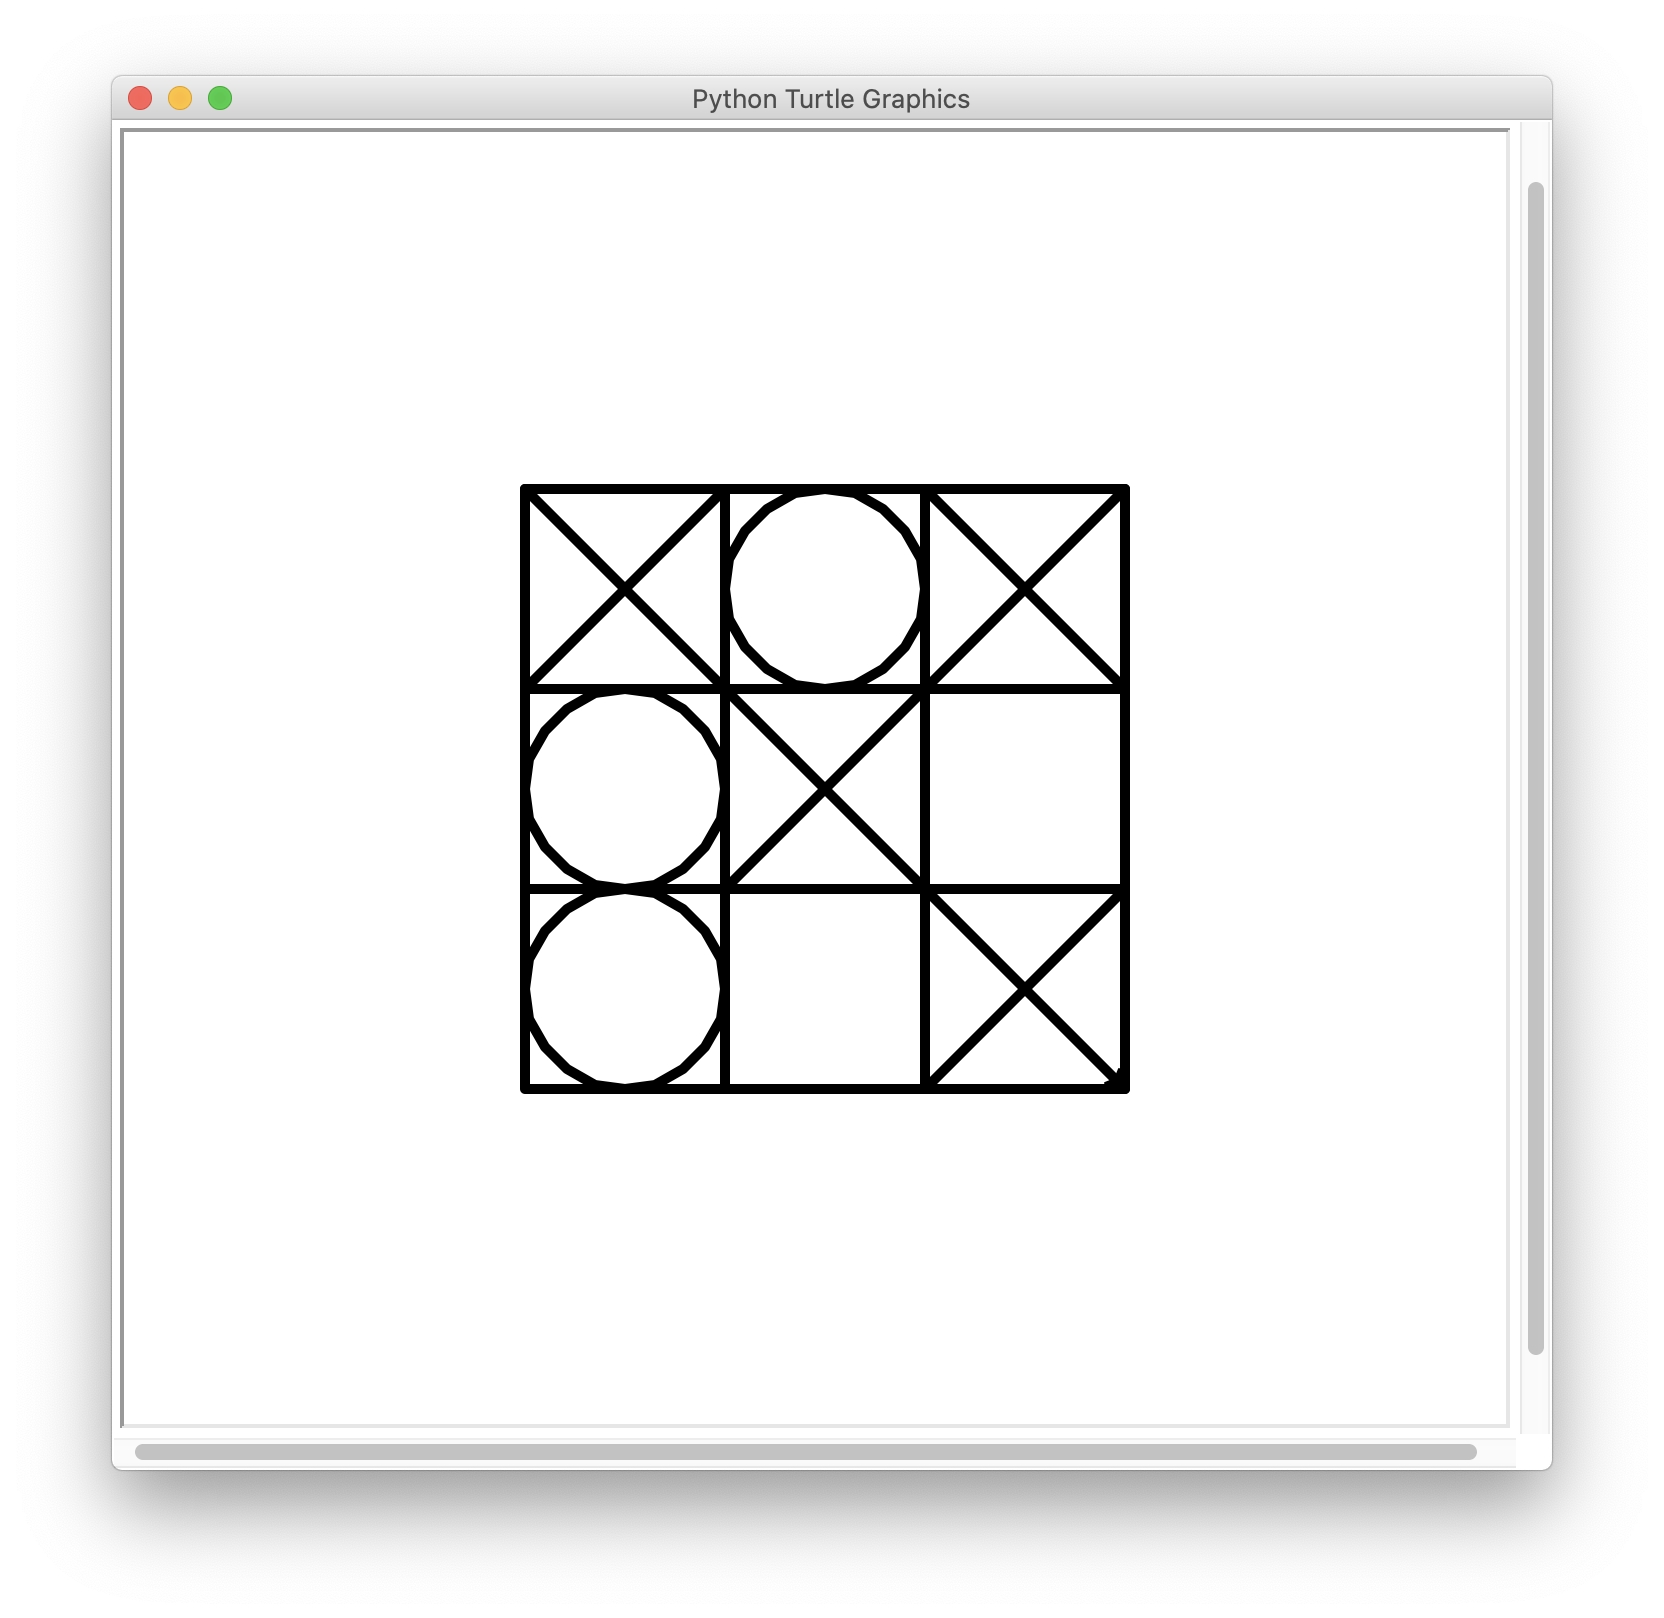
\includegraphics[width=1\textwidth]{end_game_figure.png}
\caption{Example win game image.}\label{fig:outputs}
\end{figure}

\begin{figure}[!htb]
\centering
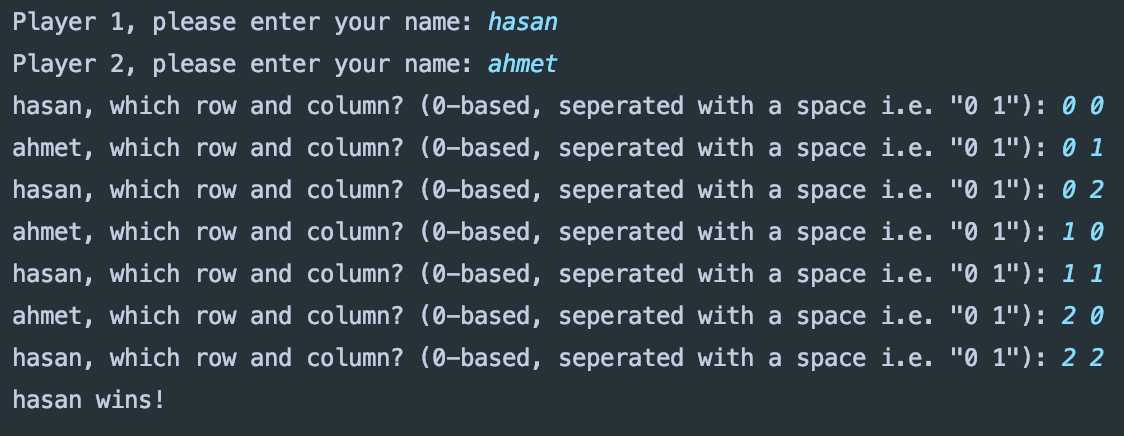
\includegraphics[width=1\textwidth]{end_game_prompt.png}
\caption{Example win game console.}\label{fig:outputs}
\end{figure}

\textbf{Hint:}
\begin{itemize}
\item A Tic-Tac-Toe win is 3 in a row - either in a row, a column, or a diagonal.
\end{itemize}


\newpage
\subsection{Congratulations!}
You reach the end of the project! If you are new to Python, this might be one of the longest programs you have written so far, so you should proud of yourself!


%Do not change this section.
\subsection{End of Project}
Your project ends here. You may continue to tinker with the code to implement any desired features and discuss them with your section leader. However, \textbf{do not} include any additional features that you implement after this point into your submission.  

\section{Resources}
You can find all course and section related material in our \href{https://koltpython.com}{website}. Also, the turtle reference below could be useful when implementing the assignment. You can find the detailed reference for turtle in \href{https://docs.python.org/2/library/turtle.html#turtle.circle}{here}. 

\subsection{Turtle Reference}
\label{themeMethod}
%This is a list. Lists always begin with this tag. "itemize" describes the list, not begin.
\begin{itemize}

%This is a list item. There is no need to indicate the end for an item as it ends at the next item tag.

\item
\begin{lstlisting}
turtle.penup()
\end{lstlisting}
Pull the pen up – no drawing when moving.

\item
\begin{lstlisting}
turtle.pendown()
\end{lstlisting}
Pull the pen down – drawing when moving.

\item
\begin{lstlisting}
turtle.forward(distance)
\end{lstlisting}
\textbf{distance} – a number (integer or float) \newline
Move the turtle forward by the specified \textit{distance}, in the direction the turtle is headed.

\item
\begin{lstlisting}
turtle.left(angle)
\end{lstlisting}
\textbf{angle} – a number (integer or float) \newline
Turn turtle left by \textit{angle} units. Angle orientation depends on the turtle mode.

\item
\begin{lstlisting}
turtle.right(angle)
\end{lstlisting}
\textbf{angle} – a number (integer or float) \newline
Turn turtle right by \textit{angle} units. Angle orientation depends on the turtle mode.

\item
\begin{lstlisting}
turtle.circle(radius)
\end{lstlisting}
\textbf{radius} – a number (integer or float)\newline
Draw a circle with given \textit{radius}. 

\item
\begin{lstlisting}
turtle.setpos(x, y)
\end{lstlisting}
\textbf{x} – a number (integer or float) \newline
\textbf{y} – a number (integer or float) \newline
Move turtle to an absolute position. If the pen is down, draw line. Do not change the turtle’s orientation.


\item
\begin{lstlisting}
turtle.setheading(to_angle)
\end{lstlisting}
\textbf{to\_angle} – a number (integer or float) \newline
Set the orientation of the turtle to \textit{to\_angle}. Here are some common directions in degrees

\end{itemize}



\end{document}